\section{\sys design}
\subsection{Overview}

\begin{figure*}[!t]
    \centering
    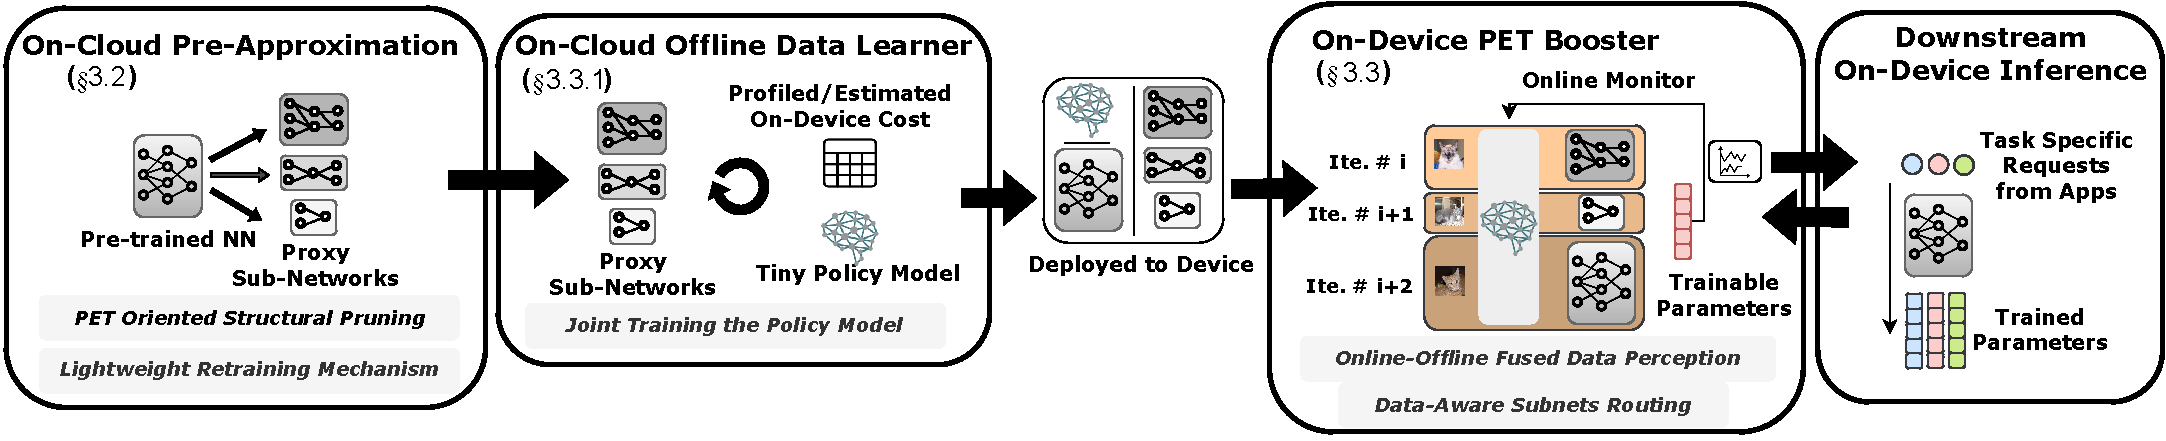
\includegraphics[width=0.995\textwidth]{figs/system_overview.pdf}
    \caption{An overview of \sys.}
    \label{fig:overview}
\end{figure*}


\noindent \textbf{System design goal.}
\sys is a cloud-device collaborated framework that aims to speed up the parameter-efficient on-device fine-tuning while not compromising the convergence accuracy (i.e., better time-to-accuracy) and the parameter efficiency.
% The key idea is to route ``easier'' and ``less-important'' data samples to more lightweight sub-networks that replace the ones in original NN that are frozen during fine-tuning.
% %through pre-generating lightweight proxy sub-networks on cloud and offloading heterogeneous training data to these proxies during on-device training.
% We refer to these lightweight sub-networks as ``proxy sub-networks'', or ``subnets'' in short, denoted by $\{F_{n}\}, n \in \{1, 2, \cdots, N\}$.
% To this end, \sys's design centers around two key questions:
% (1) At offline, how to generate lightweight and effective proxy sub-networks that well approximate the original ones?
% (2) During training, how to dynamically route heterogeneous training data to the proper proxy sub-networks?

% \mwx{define sub-network somewhere.}

\noindent \textbf{Workflow.}
Figure ~\ref{fig:overview} illustrates the two-stage simplified workflow of \sys.

At cloud offline stage, \sys generates proxy networks and prepares for the on-device training.
\ding{172} It first employs a PET oriented structured pruning to reduce the size of a given well-pre-trained original neural network. 
% It progressively removes neurons and layers, generating a series of smaller neural networks compared to the original model, i.e., \textit{proxy sub-networks}.
\ding{173} In order for the proxy sub-networks to participate in the training of the original network, a lightweight retraining mechanism is introduced to enable them to share the same latent space.
\ding{174} \sys profiles or estimates their actual on-device execution cost (including the original network) and records it in a latency score table.
% \mwx{only forward time is needed?}
% \yws{actually it's just a way to force the policy model to prefer lighter sub-networks. In my code I profiled the forward latency to realize it.}
\ding{175} Data difficulty is learned offline by an extremely lightweight end-to-end policy model.
\sys jointly trains it with the original network, proxy sub-networks, and on-device cost information using general public data on cloud.
% minimize the data selection overhead during on-device training, \sys also pre-trains a mini policy network on cloud.
% This policy network transfers the difficulty information learned from cloud data to device data basing on the assumption that the cloud pre-training data is sufficiently complex to reflect the general patterns of data distribution in the real world.
\ding{176} Finally, the original network, proxy sub-networks, and the policy model are all deployed together onto the device.

At device online stage, like other on-device continuous machine learning systems, \sys consists of two loosely-coupled runtimes, i.e., training runtime and inference runtime.
At training runtime, the plug-and-play trainable parameters are fine-tuned with device-collected data to adapt it to the drifted task or domain.
At inference runtime, the deployed NN serves as a one-size-fits-all foundation model shared by various applications.
\sys focuses on training runtime.
It dynamically routes training samples to different networks (the original network or the proxy sub-networks) according to an importance-and-difficulty-aware strategy.
This routing strategy for certain data sample $x$ is fused from two sources:
(1) The difficulty-based routing strategy from the policy model;
(2) The importance $\psi(x, t)$ monitored in near real-time.
% At this stage, we also perform opportunistic data skipping to avoid futile computation.
%takes into account the importance and difficulty of training data, dynamically routing different training data to the proper proxy networks. 
%It first inserts new trainable layers into the original NN before on-device training if necessary. 
% During the training process, it samples training data from the output of the policy network and selectively skips backpropagation based on the real-time importance of the training samples.
% Meanwhile, the importance of training samples will be fed back to the selection strategy of the proxy networks.


% \noindent \textbf{Key techniques.}
% While data diversity has been extensively studied for training optimizations ~~\cite{mercury2021sensys, guo2019spottune, 9888761, johnson2018training, katharopoulos2017biased}, we are the first to integrate it with neural sub-networks approximation to speed up on-device parameter-efficient training.
% \sys incorporates the following key techniques:
% (1) \textit{On-cloud pre-approximation}, which features a PET oriented pruning specification and a lightweight retraining mechanism ($\S$\ref{subsec:proxy network generation});
% (2) \textit{Data-aware proxy sub-networks routing}, which performs an edge-friendly online-offline fused data perception and dynamically routes data to appropriate sub-networks during on-device training ($\S$\ref{subsec:data-aware training});
% (3) \textit{Offline data difficulty learning}, which pre-learns data difficulty through a novel offline joint training method ($\S$\ref{subsubsec:policy model}).

\subsection{On-Cloud Pre-Approximation}
\label{subsec:proxy network generation}

% \begin{table}[!t]
\caption{Pruning space of different NN architectures.}
\label{table-pruning space}
\centering
    \smaller[2]
        \setlength{\tabcolsep}{1mm}{
        \begin{tabular}{c|c}
        \hline
            \textbf{Architecture} & \textbf{Pruning space} \\  
        \hline
             CNN & channels/layers \\
             Transformer & hidden sizes/attention heads/layers \\
        \hline
        \end{tabular}}
    
    
\end{table}


\textbf{Independent-Dimension Constrained (IDC) pruning.}
% the step size of pruning? the number of pruned networks?
There are many ways to obtain a lightweight approximation of the original network, such as pruning ~\cite{torchpruninggithub, huang2018multiscale}, quantization ~\cite{frantar2023gptq}, distillation ~\cite{aguilar2020knowledge}, and early exit ~\cite{xin-etal-2020-deebert}.
Intuitively, magnitude-based pruning provides the best trade-off between accuracy and computation among the above methods, since it is the most fine-grained.
Given a neural network with weights denoted as $W$, we can rank its element $w_{i}^{j}$ by the magnitude $\left\| \nabla l(x; w_{i}^{j})\cdot w_{i}^{j} \right\|$ on calibration samples $x$ and prune it.
Akin to prior arts~\cite{ma2023llmprunerstructuralpruninglarge, fang2023depgraphstructuralpruning}, \sys derives calibration samples from public general dataset (100 samples from ImageNet, by default).

To achieve actual speedup on device processors (e.g., ARM CPUs~\cite{HuaWei, mi10} or NVIDIA edge GPUs~\cite{tx2}) which typically do not support sparsity, the pruning must be structured.
However, traditional on-device acceleration oriented structured pruning~\cite{ofagithub, torchpruninggithub} lacks additional structural constraints, resulting in the approximated network being unable to participate in PET alongside the original network.
Figure~\ref{fig:pruning} shows an example of removing 20\% parameters from a PET structure in CNN.
A tuple (128, 128) represents the input/output dimensions of a layer.
If we arbitrarily prune any dimensions of a frozen layer (Figure~\ref{fig:pruning}(a)), the generated subnets cannot replace each other due to shape mismatch.

% \mwx{
% Clarify the novelty. Maybe re-organize this.
% }
To this end, \sys employs a dedicated pruning specification for PET, named Independent-Dimension Constrained (IDC) pruning (Figure~\ref{fig:pruning}(b)). 
Specifically, Given a PET network structure, IDC pruning identifies dimensions that are independent to its trainable blocks.
For a CNN block $y = \mathcal{C}_{r}(\cdots\mathcal{C}_{1}(x))$ where $\mathcal{C}_{r}(x)$ represents the $r_{th}$ convolutional layer, the independent dimensions are (1) $\mathcal{C}_{1}^{out}$, $\mathcal{C}_{2}^{in}$, $\cdots$, $\mathcal{C}_{r-1}^{in}$, if r is odd;
(2) $\mathcal{C}_{1}^{out}$, $\mathcal{C}_{2}^{in}$, $\cdots$, $\mathcal{C}_{r}^{in}$, if r is even.
For a Transformer block y = {\footnotesize $\mathcal{W}_{down}(\mathcal{W}_{up}(\mathcal{W}_{O}($$\mathcal{W}_{Q}(x)\mathcal{W}_{K}(x)\mathcal{W}_{V}(x))))$}, the independent dimensions are {\footnotesize $\mathcal{W}_{Q}^{out}$, $\mathcal{W}_{K}^{out}$, $\mathcal{W}_{V}^{out}$, $\mathcal{W}_{O}^{in}$, $\mathcal{W}_{up}^{out}$, $\mathcal{W}_{down}^{in}$}.
Following the above constraints, \sys performs magnitude-based pruning at a step size $d$ (by default 10\%, varied in $\S$\ref{subsec: sensitivity}).
For instance, proxy sub-network $\mathcal{F}_{1}$/$\mathcal{F}_{5}$ removes 10\%/50\% parameters compared to the original network $\mathcal{F}_{0}$ (and FLOPs are reduced in proportion).

% As shown in Figure ~\ref{fig:pruning}, given an original NN $\mathcal{F}_{0}$, \sys gradually performs structured pruning on its frozen parts with a step size of $d$.
\begin{figure}[!t]
    \centering
    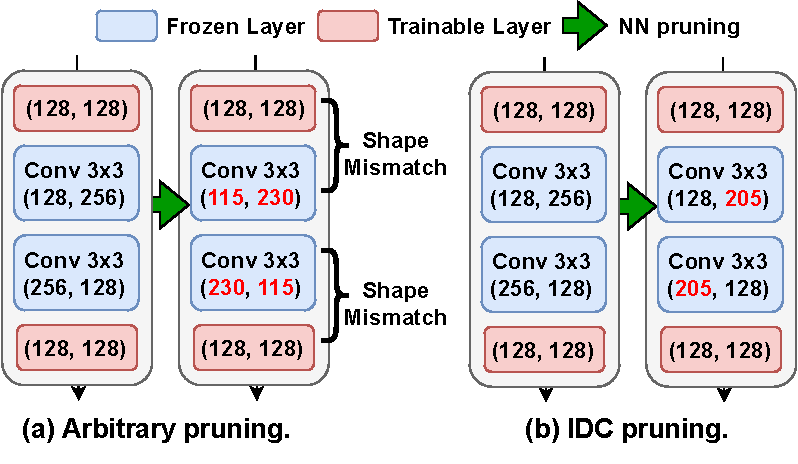
\includegraphics[width=0.88\linewidth]{figs/pruning.drawio.pdf}
    
    \caption{\sys only prunes independent dimensions of NNs. In doing so, proxy sub-networks are compatible with each other.}
    
    \label{fig:pruning}
\end{figure}

% \begin{table}[]
\footnotesize
\begin{tabular}{|l|l|}
\hline
Frozen Block &
  Independent Dimensions \\ \hline
y = $\mathcal{C}_{r}(\cdots\mathcal{C}_{1}(x))$ &
  \begin{tabular}[c]{@{}l@{}}$\mathcal{C}_{1}^{out}$, $\mathcal{C}_{2}^{in}$, $\cdots$, $\mathcal{C}_{r-1}^{in}$, if r is odd;\\ $\mathcal{C}_{1}^{out}$, $\mathcal{C}_{2}^{in}$, $\cdots$, $\mathcal{C}_{r}^{in}$, if r is even;\end{tabular} \\ \hline
\begin{tabular}[c]{@{}l@{}}y = $\mathcal{W}_{down}(\mathcal{W}_{up}(\mathcal{W}_{O}($\\ $\mathcal{W}_{Q}(x)\mathcal{W}_{K}(x)\mathcal{W}_{V}(x))))$\end{tabular} &
  \begin{tabular}[c]{@{}l@{}}$\mathcal{W}_{Q}^{out}$, $\mathcal{W}_{K}^{out}$, $\mathcal{W}_{V}^{out}$, \\ $\mathcal{W}_{O}^{in}$, $\mathcal{W}_{up}^{out}$, $\mathcal{W}_{down}^{in}$\end{tabular} \\ \hline
\end{tabular}
\end{table}

% \sys removes either some neurons of a layer (e.g., layers $b$ and $c$ in Figure ~\ref{fig:pruning}) or even the entire layer (e.g., layer $a$ in Figure ~\ref{fig:pruning}) based on the step size $d$.
% In detail, for convolution-based networks like ResNet and MobileNet, we remove channels; for Transformer-based networks like ViT, we reduce the hidden size of the MLP.
% We mainly verifies \sys on CNN and Transformer architectures, and their pruning space is as follows: 
% For CNNs (e.g., ResNet, MobileNet), we remove channels and even layers; For Transformers (e.g., ViT), we remove hidden sizes and also even layers.
% Structured removal of neurons leads to mismatched tensor shapes.
% In Figure ~\ref{fig:pruning}, ($b_{in}, b_{out}$) represent the input/output shape of a layer/block. 
% after pruning, two matrices $W_{in} \in \mathbb{R}^{n_{p}^{(l+1)} \times d_{in}^{(i)}}$ and $W_{out} \in \mathbb{R}^{d_{out}^{(i)} \times m_{p}^{(l+2)}}$ are added before/after each trainable layer separately to ensure the sharing of trainable layers across proxy networks with different shapes.
% After pruning, the output shape $b_{out}^{p}$ of layer $b$ does not match the input shape of the trainable block. 
% \sys introduces two matrices $W_{in} \in \mathbb{R}^{b_{out}^{p} \times b_{out}}$ and  $W_{out} \in \mathbb{R}^{c_{in} \times c_{in}^{p}}$ for each plugged PET block.
% $n^{(l)}$ and $m^{(l)}$ represent the output/input dimensions of the $l_{th}$ frozen layer, and $n_{p}^{(l)}$ and $m_{p}^{(l)}$ are the output/input dimensions after structural pruning. 
% $d_{in}^{(i)}$ and $d_{out}^{(i)}$ represent the input/output dimensions of the $i_{th}$ trainable layer.
% Note that the computational cost of $W_{in}$ and $W_{out}$ is also considered in the pruning step size $d$.
% In practice, we prefer to remove more parts from the layers closer to the network output.
In a nutshell, \sys's IDC pruning effectively provides approximations that achieve on-device speedup, and enables the generated proxy subnets to work seamlessly with each other.

% \noindent \textbf{Comparing IDC pruning with other approximations.}
% \mwx{
% (1) compared with pruning. (2) 
% }

\begin{figure}[!t]
	\centering
	\subfloat[Visualized feature\label{fig:shifting1}]{%
  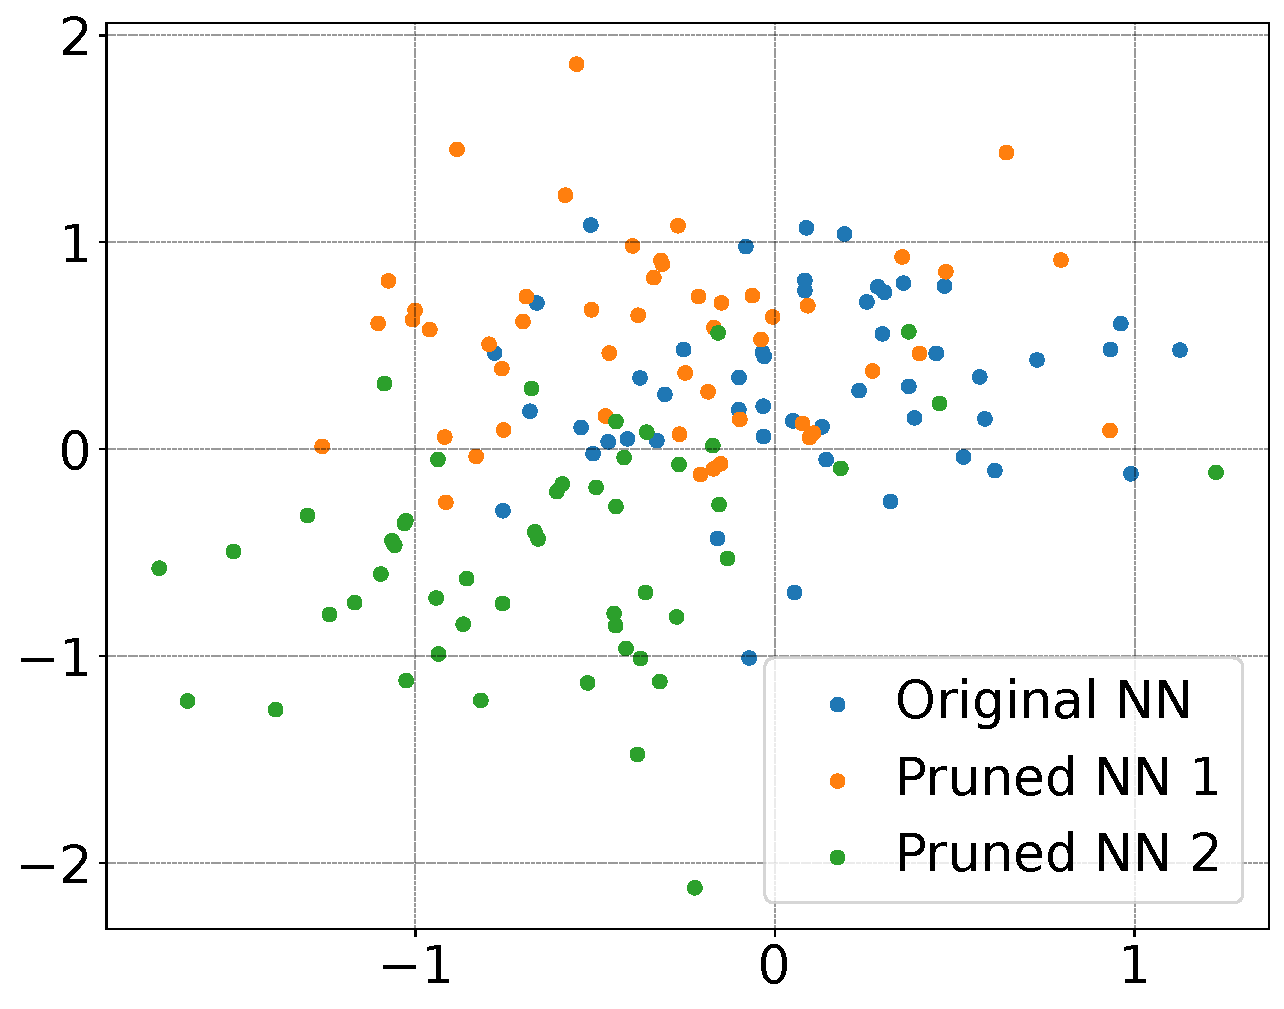
\includegraphics[width=0.45\linewidth]{figs/shifting1.pdf}}
	\subfloat[Vanilla FT vs. ours\label{fig:shifting2}]{%
  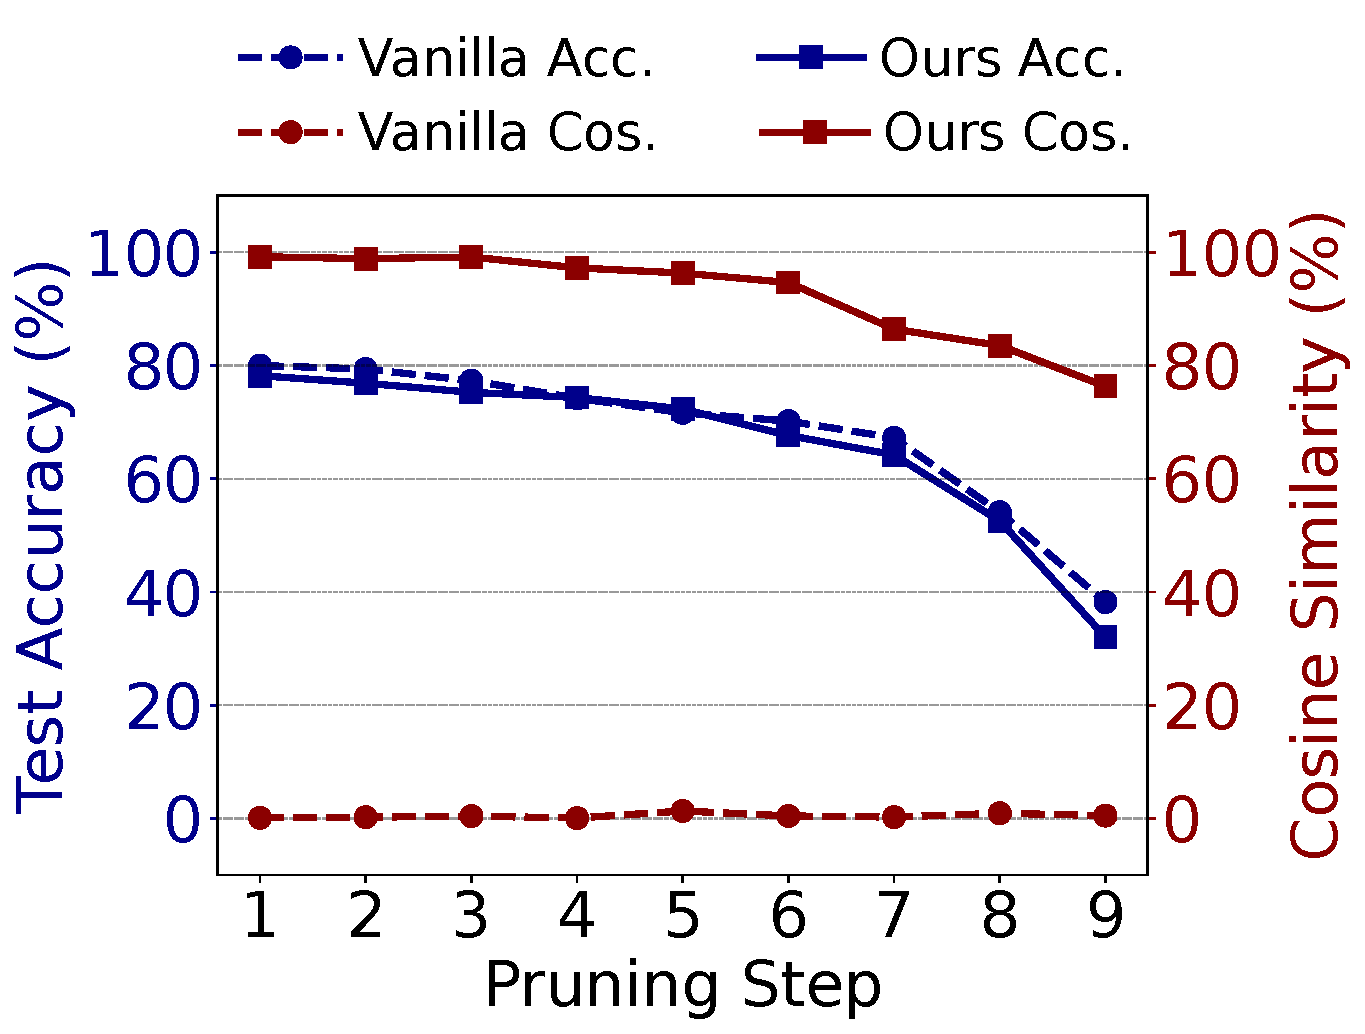
\includegraphics[width=0.51\linewidth]{figs/shifting2.pdf}}

	\caption{The latent space shift.
        (a) The visualized feature extracted by the original NN and 2 pruned subnets suffers a shift.
        (b) Test Accuracy and average cosine similarity between pruned and original NN.}
\end{figure}

\noindent \textbf{Latent space alignment through lightweight retraining.}
Unfortunately, the proxy sub-network pruned by IDC pruning is still not a good (accurate) approximation.
We dive into the reason and find out that the requirements of NN approximation for training are more stringent.
In Figure ~\ref{fig:shifting1}. we reduce the dimensionality of the latent space through PCA (Principal Component Analysis) and visualize it.
The latent spaces exhibit a gap.
It means that, though the pruned network may retain the ability to do inference (e.g., predict a dog as ``dog''), the feature feed to the shared trainable block may be tortured and thus noisy for PET.
To this end, we propose an enhanced alignment method with a dedicated regularization term. 
For each proxy sub-network $\mathcal{F}_{n}$, $n \in \{1, 2, \cdots, N\}$, we respectively minimize
% not a formula, too. formulize it latter.
% \begin{align}
% 	\mathcal{L} = -\sum_{i=1}^{k} y_i \log \left( \frac{e^{z_i}}{\sum_{j=1}^{k} e^{z_j}} \right) + \sum_{r=1}^{R}\lambda_{r} (h_{0}^{r} \otimes  h_{n}^{r}),
% 	\label{eq-loss_cosine_finetune}
% \end{align}
\begin{align}
%
	\mathcal{L} = \mathcal{L'} + \sum_{r=1}^{R}\lambda_{r} (h_{0}^{r} \otimes  h_{n}^{r}),
%
	\label{eq-loss_cosine_finetune}
\end{align}
where $\mathcal{L'}$ is vanilla fine-tuning loss (e.g. cross entropy loss), $h_{n}^{r}$ is the hidden state before the $r_{th}$ trainable block (i.e., the input), $R$ is the number of trainable blocks, $ \otimes $ is an operator to compute similarity, and $\lambda_{r}$ is the scale factor (1.0 by default).
% $L_{CoE}$ is the cosine-embedding loss function, and $h_{j}^{i}$ represents the activation of the $i_{th}$ trainable layer of the $j_{th}$ proxy network.
% $\lambda_{i}$ is the scale factor, and $I$ is the number of trainable layers.
% We use cosine similarity to measure the similarity between $h_{0}^{r}$ and $h_{n}^{r}$.
% , i.e.,
% \begin{align}
%         h_{0}^{r} \otimes h_{n}^{r} = \frac{h_{0}^{r} \cdot h_{n}^{r}}{ \left\| h_{0}^{r} \right\| \left\| h_{n}^{r} \right\|}.
% \end{align}
% It is easier to converge compared to  mean squared error (MSE) from our observation.
\textbf{\textit{Effectiveness}.}
\yws{
Figure ~\ref{fig:shifting2} reports the test accuracy and latent space alignment of vanilla fine-tuning and our method.
After vanilla fine-tuning, the features can only maintain a good test accuracy but compromise the alignment, while our method achieves both.
We integrate our alignment method into a lightweight retraining mechanism triggered after pruning.
We also conduct experiments on significance of key designs in $\S$\ref{subsec: sensitivity}. 
}
% \mwx{
% Clarify the novelty.
% }


% \mwx{Add the following parts: }

% \noindent \textbf{Necessity and novelty of the key designs.}
% \mwx{
% (1) Necessity of IDC pruning. Without 
% }

\noindent \textbf{Overhead analysis.}
Firstly, it is worth noting that the pre-approximation process takes place on cloud, which is relatively resource-abundant.
Secondly, compared to the resource-intensive pre-training process, the cost of our pruning and retraining is much lower.
We only perform 3 epoch of retraining for each sub-network.
% For instance, pruning and retraining 10 proxy sub-networks for a ResNet50 consumes just 1\%-10\% additional GPU hours. 
Furthermore, this process is executed one-shot: these approximated public proxy sub-networks can be shared by various devices.

\subsection{On-Device Data-Aware Routing}
\label{subsec:data-aware training}

\noindent \textbf{Profiling data diversity: undesirable system overhead.}
According to equation ~\ref{eq-difficulty_def}, acquiring the difficulty of a training sample is ``posterior'': it demands up to $N$ forward passes in the worst case (whereas the training itself involves just one forward/backward pass), which is unacceptable on devices.
According to equation ~\ref{eq-importance_def}, data importance is ``stateful'': it is influenced by the current training state $t$, which incurs additional forward computations~\cite{mercury2021sensys} for accurate perception because of the issue of ``staleness'' (Figure ~\ref{fig:stale}).

\noindent \textbf{Online-offline fused data perception.}
Inspired by ML-based system optimization efforts, such as database query optimization~\cite{marcus2021bao, negi2021steering} and matrix multiplication optimization~\cite{fawzi2022discovering}, we decouple the perception of data difficulty to the on-cloud offline phase.
Specifically, we design a data-driven black-box tiny model, referred as policy model $\Omega$.
The model is offline trained and performs online inference.
The design and training details are shown in $\S$\ref{subsubsec:policy model}.
As a stateful attribution, data importance is still perceived online.
We use the current forward pass to get real-time data importance.
\yws{
At a certain iteration, the importance comes from the current network state by reusing the training loss, and the details are presented in the following Algorithm~\ref{alg:on-device_training}.
}
% \mwx{Elaborate what the ``hitchihike'' means here.}

The above online-offline fused data perception incurs negligible online overhead.
Most of the additional overhead comes from the online inference of the tiny policy model.
For instance, on NVIDIA Jetson TX2, the per-sample perception time for ResNet50 is only 0.6 ms on average, which is less than 1\% of an entire training iteration.

\begin{figure}[!t]
    \centering
    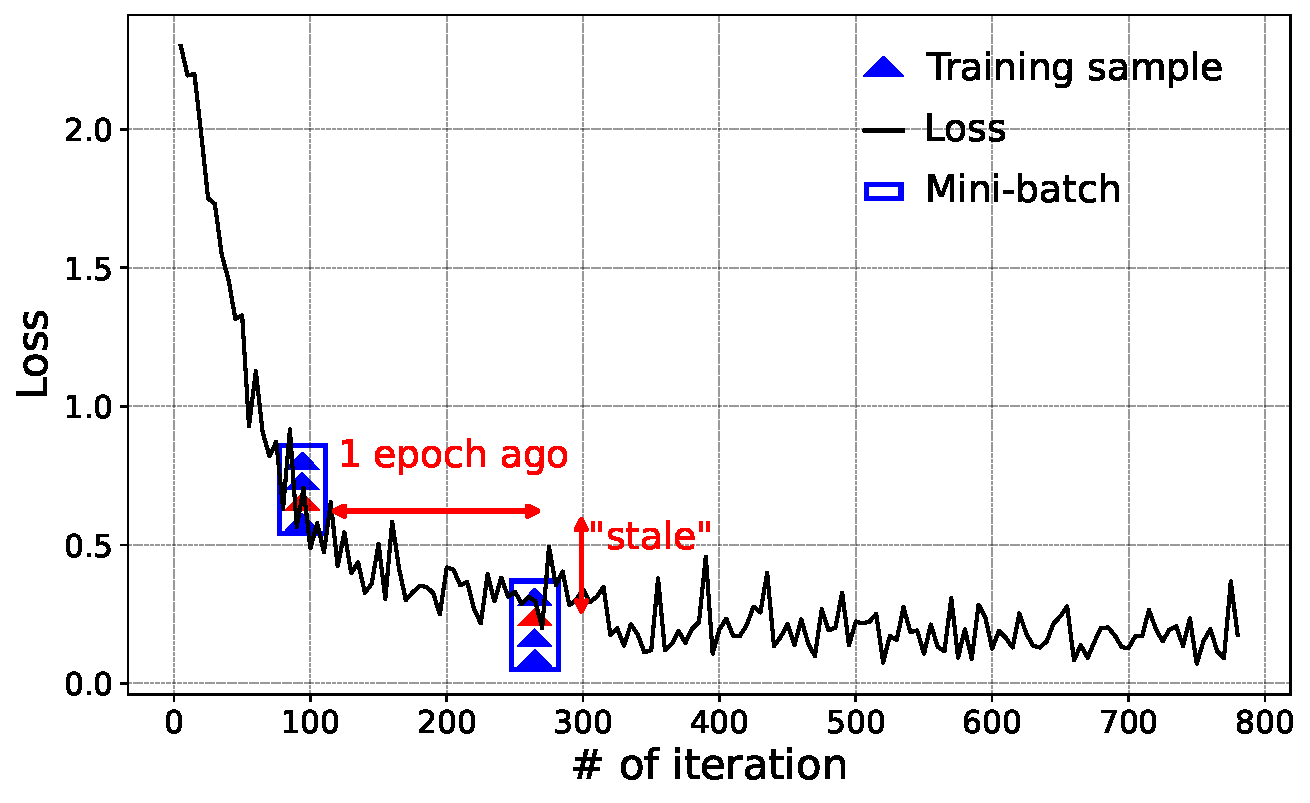
\includegraphics[width=0.82\linewidth]{figs/stale.pdf}
    \caption{The precision of data importance estimation. The estimate of specific training sample (red triangle) from the previous forward pass becomes ``stale'' as the training progresses.}
    \label{fig:stale}
\end{figure}

\begin{algorithm}[t]
\scriptsize
\SetAlgoNlRelativeSize{-1}
% \SetAlgoNlRelativeSize{-3}
\SetAlgoNoEnd
\SetKwProg{Fn}{Function}{~}{end}
\SetKwInOut{Input}{input}\SetKwInOut{Output}{output}\SetKwInOut{Variable}{Variable}
\Input{\footnotesize
    \textcolor{blue!85!black}{$\{\mathcal{F}_{n}\}$}, $n \in \{0, 1, 2, \cdots, N\}$; \textcolor{blue!85!black}{$\Omega$}; On-device dataset \textcolor{blue!85!black}{$D$};
}
\Output{\footnotesize
    Fine-tuned \textcolor{blue!85!black}{$\mathcal{F}_{0}$};
}
\BlankLine
\Fn{\footnotesize \textcolor[RGB]{170,144,6}{data\_aware\_training():}}{
    % $loss\_func$ \textcolor{red!85!black}{$\leftarrow$} $CrELoss()$; 
    % \tcc{Initialization}
    \textcolor{blue!85!black}{$train\_loader$} \textcolor{red!85!black}{$\leftarrow$} \textcolor{blue!85!black}{$D$}, \textcolor[RGB]{170,144,6}{$Policy\_sampler()$};
    \textcolor{blue!85!black}{$\theta$} \textcolor{red!85!black}{$\leftarrow$} \textcolor{green!50!black}{$-1$}; 
    \textcolor{blue!85!black}{$m$} \textcolor{red!85!black}{$\leftarrow$} \textcolor{green!50!black}{$0.8$}\;
    \For{\textcolor{blue!85!black}{$epoch$} \textbf{in} \textcolor{blue!85!black}{$epochs$}}{
        \For{ \textcolor{blue!85!black}{$data$} \textbf{in} \textcolor{blue!85!black}{$train\_loader$}}{
            \textcolor{blue!85!black}{$X$}, \textcolor{blue!85!black}{$n$} \textcolor{red!85!black}{$\leftarrow$} \textcolor{blue!85!black}{$data$}; \textcolor{green!60!black}{\tcp{mini-batch and routing strategy}}
            \textcolor{blue!85!black}{$l$} \textcolor{red!85!black}{$\leftarrow$} \textcolor{blue!85!black}{$X$}, \textcolor{blue!85!black}{$\mathcal{F}_{n}$}; \textcolor{green!60!black}{\tcp{get loss by \textbf{one} sub-network $\mathcal{F}_{n}$}}
            \textcolor{green!60!black}{\tcc{Opportunistic data skipping}}
            \For{\textcolor{blue!85!black}{$x$} \textbf{in} \textcolor{blue!85!black}{$X$}}{
                \lIf{ \textcolor{blue!85!black}{$l[x]$} \textcolor{red!85!black}{>} \textcolor{blue!85!black}{$\theta$}}{
                    \textcolor{blue!85!black}{$l[x]$}\textcolor[RGB]{170,144,6}{$.bp()$};
                    \textcolor{blue!85!black}{$sampler$}\textcolor[RGB]{170,144,6}{.\textit{adjust}(}\textcolor{blue!85!black}{$x$}, \textcolor{green!50!black}{$0$}\textcolor[RGB]{170,144,6}{)}
                }\lElse{
                    \textcolor{blue!85!black}{$sampler$}\textcolor[RGB]{170,144,6}{.\textit{adjust}(}\textcolor{blue!85!black}{$x$}, \textcolor{green!50!black}{$1$}\textcolor[RGB]{170,144,6}{)}
                }
            } 
            \textcolor{green!60!black}{\tcc{Momentum-based filtering threshold}}
            \textbf{if} \textcolor{blue!85!black}{$\theta$}==\textcolor{green!50!black}{$-1$} \textbf{then} \textcolor{blue!85!black}{$\theta$} \textcolor{red!85!black}{$\leftarrow$} \textcolor{blue!85!black}{$l$}; \textbf{else} \textcolor{blue!85!black}{$\theta$} \textcolor{red!85!black}{$\leftarrow$} \textcolor{blue!85!black}{$m\theta$} + \textcolor{blue!85!black}{$(1-m)l$}\;
            \textcolor{green!60!black}{\tcc{Synchronizing trainable blocks}}
            \textbf{for} \textcolor{blue!85!black}{$i$} \textbf{in} \textcolor{blue!85!black}{\{0, 1, $\cdots$, $N$\}} \textbf{ do } \textcolor{blue!85!black}{$\ensuremath{\mathcal{F}_{i}}$} \textcolor{blue!85!black}{$.trainable$} \textcolor{red!85!black}{$\leftarrow$} \textcolor{blue!85!black}{$\ensuremath{\mathcal{F}_{n}}$} \textcolor{blue!85!black}{$.trainable$};
        }
    }
    \textbf{return} \textcolor{blue!85!black}{$\ensuremath{\mathcal{F}_{0}}$};
}
% \Fn{\footnotesize{\textcolor[RGB]{170,144,6}{Policy\_sampler():}} \scriptsize{\textcolor{green!60!black}{\tcp{called once per epoch}}}}{
%     aaa
% }

\Fn{\footnotesize{\textcolor[RGB]{170,144,6}{Policy\_sampler():}} \scriptsize{\textcolor{green!60!black}{\tcp*[h]{called once per epoch}}}}{
    \textcolor{blue!85!black}{$P$} \textcolor{red!85!black}{$\leftarrow$} \textcolor{blue!85!black}{$\Omega$}, \textcolor{blue!85!black}{$D$}; \textcolor{green!60!black}{\tcp{a list, routing strategy $n$ = $P$[index of $x$]}}
    \Fn{\footnotesize{\textcolor[RGB]{170,144,6}{adjust(\textcolor{blue!85!black}{$x$}, \textcolor{blue!85!black}{$\epsilon$})};} \scriptsize{\textcolor{green!60!black}{\tcp*[h]{adjust $x$'s routing strategy by $\epsilon$}}}}{}
    % $policy\_list$ \textcolor{red!85!black}{$\leftarrow$} adjust the $policy\_list$ based on the filter \; 
    \textcolor{blue!85!black}{$Q$} \textcolor{red!85!black}{$\leftarrow$} \textcolor{blue!85!black}{$[0:\textcolor[RGB]{170,144,6}{len(}D\textcolor[RGB]{170,144,6}{)}]$}; \textcolor{green!60!black}{\tcp*[h]{a list storing sampling order of $D$}} \\
    \textcolor{blue!85!black}{$Q$}\footnotesize{\textcolor[RGB]{170,144,6}{.\textit{sort}()}\textcolor[RGB]{170,144,6}{.\textit{shuffle}()}}; \scriptsize{\textcolor{green!60!black}{\tcp*[h]{sort by policy, shuffle in same policy}}} \\
    \textbf{return} \textcolor{blue!85!black}{$sampler$}; \textcolor{green!60!black}{\tcp*[h]{for $train\_loader$ to sample mini-batch}}
}

\caption{Data-aware on-device training.}
\label{alg:on-device_training}
\end{algorithm}



\noindent \textbf{Data-aware subnet routing.}
Based on the perceived data diversity, \sys judiciously assigns training samples to proper subnets.
In general, we obtain a difficulty-based routing strategy from the policy model, and adjust this strategy with real-time data importance.
This strategy is dynamic: during training, each mini-batch selects the most suitable sub-network for itself.

In detail, we demonstrate our routing strategy by describing the on-device training procedure of \sys in algorithm ~\ref{alg:on-device_training}.
It receives \{$\mathcal{F}_{n}$\}, $\Omega$, and the on-device dataset $D$, and finally outputs the fine-tuned network $\mathcal{F}_{0}$.
The routing strategy is maintained by function $Policy\_sampler()$, which samples mini-batches and ensures that samples within the same mini-batch share the same level of difficulty.
After getting the output of $\Omega$ (line 17), we online adjust it by function $adjust()$ (line 18, line 8--10).
Both $\Omega$ and $adjust()$ adhere to the principle of minimizing computation for easier or less important data.
% \yws{An example? not clear here.}
The main body of on-device training is in function $data\_aware\_training()$.
During each iteration, we sample a mini-batch $X$, obtain its routing strategy $n$, and select a proxy sub-network $\mathcal{F}_{n}$ for training (line 5--6).

% \mwx{Give high-level description of our routing strategy, especially how data difficulty and importance affect the routing.}

% \mwx{Focus on following questions: at high level, why the data difficulty needs to be learned, while importance does not? How data importance is calculated (data difficulty details can go later)?}

% \noindent \textbf{Opportunistic Data Skipping.}
% \begin{figure}[!t]
    \centering
    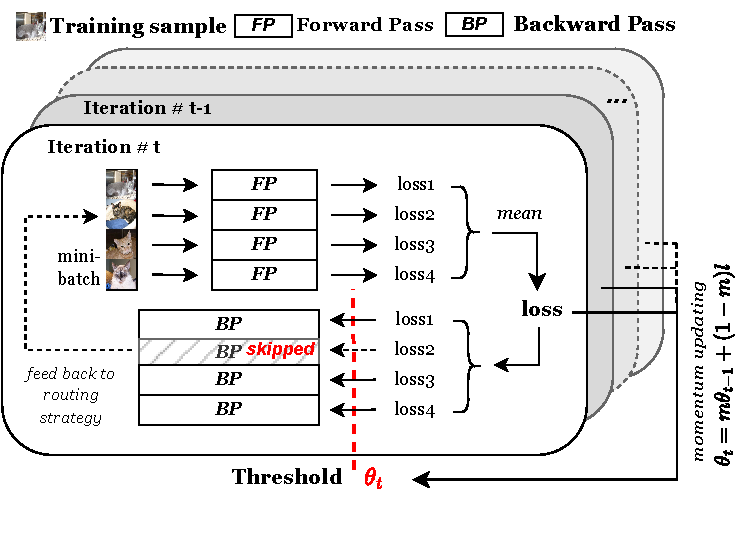
\includegraphics[width=0.82\linewidth]{figs/importance_filter.pdf}
    
    \caption{\sys opportunistic data skipping.}
    \label{fig:filter workflow}
    
\end{figure}

% \noindent \textbf{Skipping . }
In line 7--12, we further filter unimportant data from back-propagation.
Training data that has already well converged is all pain and no gain: it consumes computational resources while contributes little to convergence.
% Fortunately, our design of data-aware subnets routing has provided us with the opportunity to skip over these data points when profiling data importance.
%As shown in Figure ~\ref{fig:filter workflow}, 
We skip the backward pass stage of training sample $x$ by comparing its data importance to a threshold $\theta$.
To perform stable and solid filtering, $\theta$ is dynamically updated based on momentum.
Let $\theta_{t}$ be the threshold at iteration $t$, $m\in[0, 1)$ be the momentum coefficient, $l$ be the loss of current iteration, then we get
\begin{align}
	\theta_{t+1} = m\theta_{t} + (1-m)l.
	\label{eq-filter_thres}
\end{align}
Usually, $\theta$ is initialized as the loss from the first iteration, and $m$ is relatively large (e.g., 0.8, our default).
After filtering, we then feed the profiled importance back to routing strategy by function $adjust()$.

\noindent \textbf{Asynchronous subnets loading. }
Notably, only \textit{one} proxy sub-network is involved in a training iteration, so keeping all networks in device memory simultaneously is not necessary.
Thereby, \sys asynchronously loads the subnet of next iteration during the current iteration.
Such a loading is overhead-free in training time as computation time is much longer than loading.
% \mwx{About 0.8 page. Move Sec 3.5 \& 3.6 here.}
In doing so, the peak memory usage of our framework is nearly identical to PET, with only additional buffers for maintaining weights of a proxy sub-network of next iteration (detailed in $\S$\ref{subsec: energy}).

% \mwx{This paragraph is relatively independent.}

\subsubsection{\textbf{Learned Data Difficulty}}
\label{subsubsec:policy model}
Here we focus on the details of how data difficulty is obtained through offline-online collaboration.
% \mwx{Explain the following things in rationale: (1) why data difficulty can be learned (2) How does the learning work (3) Why it should be learned. Especially, the learning is also free of the need for defining the similarity constraint $\sigma$, since the feature similarity is end-to-end represented by the learning loss.}
\yws{
As discussed before, a straightforward way to perceive the data difficulty is to run all (pre-trained) proxy networks for a data sample to compare the features (recall Equation~\ref{eq-difficulty_def}).
On one hand, running all proxy networks is unacceptable on devices, and the constraint to determine whether $\mathcal{F}_{n} (x) \simeq \mathcal{F}_{0}(x)$ also involves ad-hoc designs (e.g., using cosine similarity; setting threshold $\sigma$, etc.).
On the other hand, as an intrinsic characteristic standalone to training state, intuitively the data difficulty does not have to be perceived online.
}
% \mwx{About 0.7 page. Move Sec 3.4 here. What's the cost of offline training?}

% \mwx{This section focuses on the details of how data difficulty is obtained through offline-online collaboration.}

%(为什么都有效，为什么我们同时考虑)
% \subsection{Difficulty-based Data-to-subnets Routing Policy Model}
% \label{subsec:the policy model}
% needs to be renamed, current name leads to misunderstanding.

%\textbf{The need for a lightweight routing strategy.}
% During on-device training, obtaining the difficulty $\phi(x)$ of each training sample $x$ and selecting an appropriate proxy sub-network $\mathcal{F}_{n}$ would introduce additional overhead.
% Equation ~\ref{eq-difficulty_def} already implies the inherent complexity of this issue.
% % By equation ~\ref{eq-difficulty_def}, naive approaches like directly comparing the features extracted from different proxy sub-networks result in significant computational overhead due to the need to perform forward pass for each sample on each proxy sub-network in every training iteration.
% A naive approach that directly compares the features extracted from different proxy sub-networks needs to perform a forward pass for each sample and proxy sub-network, thus incurring unacceptable overhead.
% %Taking the example of training a ResNet50 model with 1 adapter using 3 proxy sub-networks with a pruning step size of 20\%, obtaining the data difficulty for each iteration takes 168 ms, while the training process itself only takes 62 ms.

% \mwx{What's the rationale? Need more description of Fig 10 and make this technique clearer (it seems to be the most novel one).}
\noindent \textbf{``Learned data difficulty'' through a lightweight policy model.}
\yws{
\sys's response is an end-to-end learning for data difficulty with implicitly determining $\mathcal{F}_{n} (x) \simeq \mathcal{F}_{0}(x)$ by the learning loss.
}
We design a lightweight policy model $\Omega$ to end-to-end learn the data difficulty.
The input of the policy model is a training sample $x'$ downsampled from $x$ (\yws{i.e., resizing the input using interpolation}), and the output is a one-hot vector $\Omega(x') \in \mathbb{R}^{1 \times (N+1)}$. 
% \mwx{Details of downsample.}
$\Omega$ is tiny because we only use a small fraction of the original network $\mathcal{F}_{0}$. 
For instance, we use 2 residual blocks for ResNet50, 2 basic blocks with 2 depthwise separable convolutions each for MobileNetV3, or 1 encoder layer for ViT base, and each module has a smaller size compared to the original network. 
The total parameter count is less than 5\% of the original network.\footnote{
Although increasing the model size may lead to better routing performance, the benefits diminish marginally, while the online inference overhead shows no marginal effect. Therefore, we keep it small enough.}
% The size of these modules is also set to a fraction of the original model.

\begin{figure}[!t]
    \centering
    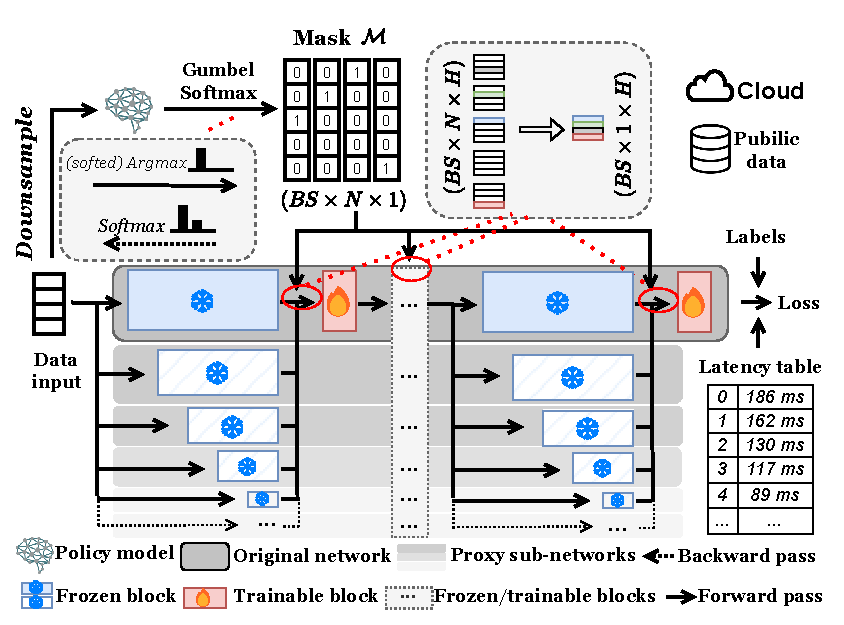
\includegraphics[width=0.98\linewidth]{figs/policy.pdf}
    \caption{Learning difficulty through joint training.}
    \label{fig:policy_model}
\end{figure}

\noindent \textbf{Joint training the policy model.}
The policy model is jointly trained with the original network and the proxy sub-networks (i.e., $\{\mathcal{F}_{n}\}, n \in \{0, 1, 2, \cdots, N\}$) on large-scale public cloud data.
% We pre-profile the proxy networks on device to obtain the realistic time consumption, and use the profiled latency during the policy model training.
The training procedure is shown in Figure ~\ref{fig:policy_model}.
We combine $\Omega$ and $\{\mathcal{F}_{n}\}$ together to create a joint end-to-end trainable network.
% Specifically, the manner in which we combine these networks is mainly demonstrated in Formula ~\ref{eq-policy_model_tuning_structure}.
The network structure before the $r_{th}$ trainable block (i.e., the red circle in Figure ~\ref{fig:policy_model}) is %can be represented by Equation ~\ref{eq-policy_model_tuning_structure}.
\begin{align}
	% y = sum(concat_{j=0}^{K}(x_{j}) \circ \mathcal{M}),
        x_{r} = \sum_{dim=1}[(x_{0}^{r}|x_{1}^{r}|\cdots|x_{n}^{r}|\cdots|x_{N}^{r}) \circ \mathcal{M}] 
	\label{eq-policy_model_tuning_structure}
\end{align}
% persudo code? formula is hard to express.
% squeeze?
where $x_{n}^{r} \in \mathbb{R}^{BS \times 1 \times H}$ is from the $n_{th}$ network $\mathcal{F}_{n}$, $\circ$ is the Hadamard product, $\mathcal{M} \in \mathbb{R}^{BS \times N \times 1}$ is the mask from the policy model, $BS$ is the mini-batch size, $N$ is the number of proxy sub-networks, $H$ is the hidden state size, $(x_{0}^{r}|x_{1}^{r}|\cdots|x_{n}^{r}|\cdots|x_{N}^{r})$ represents concatenating the tensors sequentially at the $1_{st}$ dimension, $\sum_{dim=1}$ represents summarizing the tensors along the $1_{st}$ dimension, and finally we get the input tensor $x_{r}$ of the $r_{th}$ trainable block.
% Each frozen block shares the input from the output of the previous block (usually the output of the preceding trainable block or the input to the entire model).
In addition, since the output of the policy model $\Omega$ is discrete, which makes $\Omega$ non-differentiable, we borrow the Gumbel-Softmax~~\cite{jang2017categorical} trick\footnote{An open-source implementation of Gumbel-Softmax Sampling: \url{https://github.com/gyhui14/spottune/blob/master/gumbel_softmax.py}} to facilitate the backpropagation of the gradient to the policy model.

We update the parameters of the policy model and the trainable blocks while keeping the frozen blocks frozen again.
We minimize a multi-task learning loss
% \begin{align}
% 	\mathcal{L} = -\sum_{i=1}^{k} y_i \log \left( \frac{e^{z_i}}{\sum_{j=1}^{k} e^{z_j}} \right) + \lambda \frac{1}{N}\sum_{*}(\mathcal{M} \circ \mathcal{S}),
% 	\label{eq-policy_model_tuning_loss}
% \end{align}

\begin{align}
	\mathcal{L} = \mathcal{L'} + \lambda \frac{1}{N}\sum_{*}(\mathcal{M} \circ \mathcal{S}),
	\label{eq-policy_model_tuning_loss}
\end{align}

where $\lambda$ is the scale factor (1.0 by default), $\sum_{*}$ represents summing all elements in the tensor, $\mathcal{M} \in \mathbb{R}^{N \times 1}$ is the mask tensor from the policy model, $\mathcal{S} \in \mathbb{R}^{N \times 1}$ is the on-device profiled latency scores of networks $\{\mathcal{F}_{n}\}$, $n \in \{0, 1, 2, \cdots, N\}$.
Equation ~\ref{eq-policy_model_tuning_loss} forces the policy model $\Omega$ to learn a strategy that minimizes computational complexity (the second term) while ensuring accuracy (the first term).

\noindent \textbf{Training data.}
\yws{
By default, the learning of policy model is on the large-scale general dataset used in the pre-training process (e.g. ImageNet).
Although the policy model is deployed on devices for new fine-tuning data, it shows a strong transferablity without the need for retraining the policy model in most cases, since a large-scale general training dataset has covered a wide range of difficulty patterns.
We make a detailed evaluation and discussion on the training data distribution issue in $\S$\ref{subsec: sensitivity} and $\S$\ref{subsec: discussion}.
}

% \mwx{Data distribution issue.}

\noindent \textbf{Training overhead.}
\yws{
The joint training converges within a single epoch and 
also only requires one-shot execution like the on-cloud pre-approximation.
In general, the entire training only incurs 5\%--10\% GPU-hours of the vanilla pre-training process.
}

% \subsection{Importance-based Data Skipping}
% \label{subsec:the importance filter}
% % \yws{(Shall we explain the difference between importance sampling (Mercury) and importance filtering?)}
% \mwx{This technique is not closely coupled with our key idea (proxy subnets), any idea?}
% \yws{Data importance influences routing strategy by feeding back to and modifying it. $\S$\ref{subsec:On-device training procedure} Policy\_sampler()}

% We use the feed-forward loss to estimate the importance $\mathcal{\psi}(x, t)$ of training data ~~\cite{mercury2021sensys, katharopoulos2017biased} during on-device training.
% The larger the loss, the more important the training data.
% \begin{figure}[!t]
    \centering
    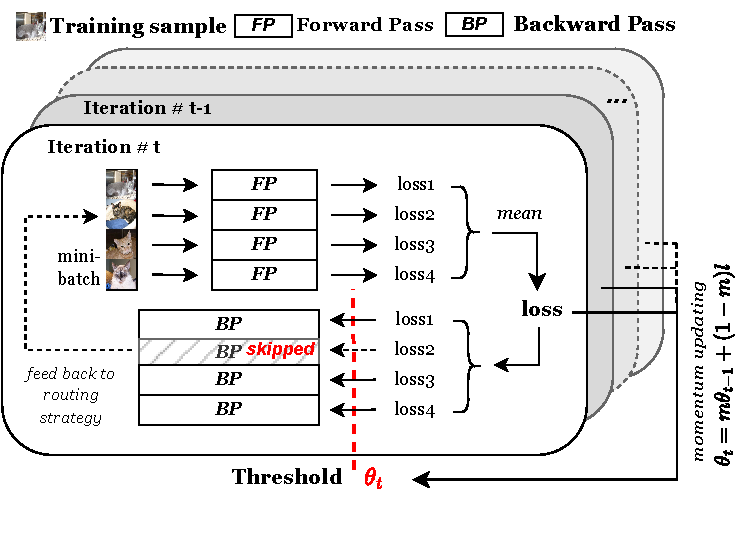
\includegraphics[width=0.82\linewidth]{figs/importance_filter.pdf}
    
    \caption{\sys opportunistic data skipping.}
    \label{fig:filter workflow}
    
\end{figure}

% \begin{figure}[!t]
    \centering
    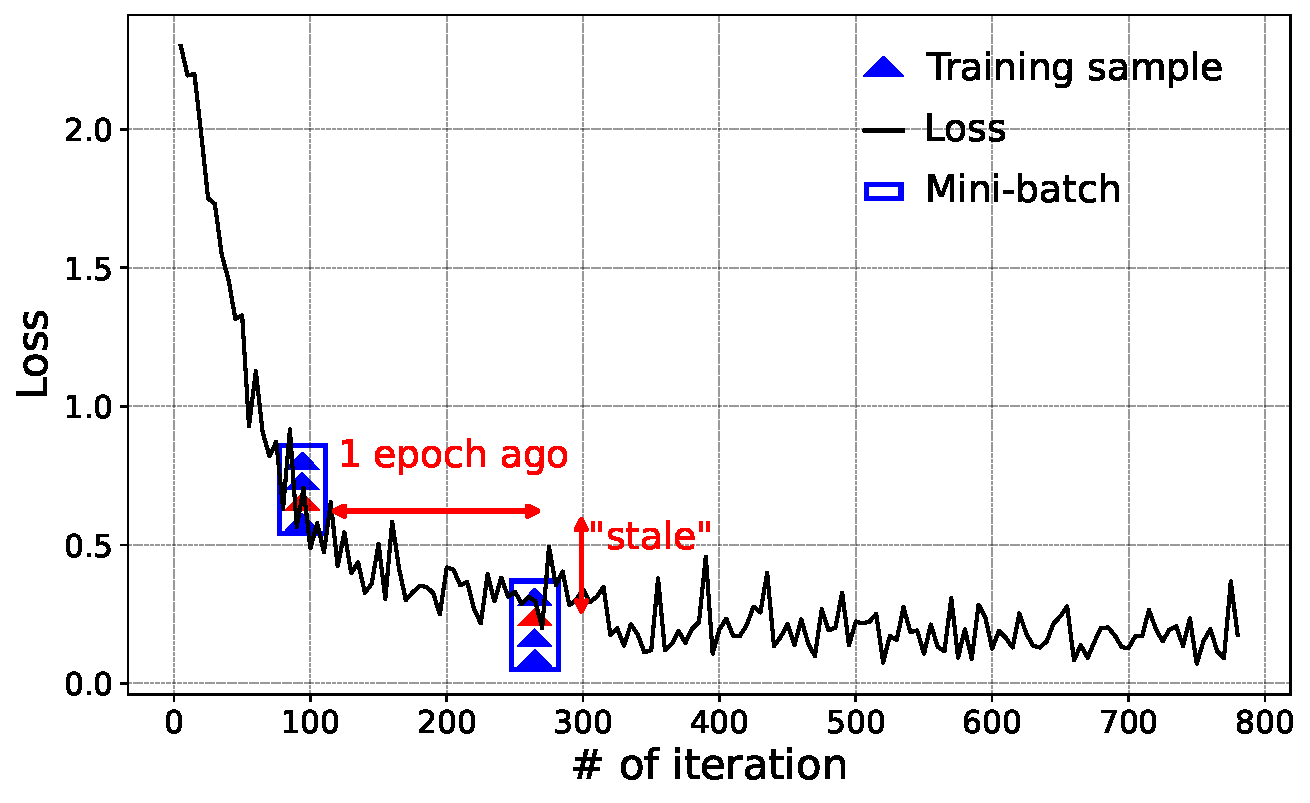
\includegraphics[width=0.82\linewidth]{figs/stale.pdf}
    \caption{The precision of data importance estimation. The estimate of specific training sample (red triangle) from the previous forward pass becomes ``stale'' as the training progresses.}
    \label{fig:stale}
\end{figure}


% \noindent \textbf{Challenges.}
% However, leveraging variations in data importance to expedite training convergence faces two challenges: (1) data importance estimation overhead; (2) precision of the estimation.
% On one hand, there are topological dependencies between various computational stages in a training iteration (Figure ~\ref{fig:filter workflow}). 
% To obtain the feed-forward loss, the forward pass must be performed first.
% On the other hand, since the NN weights are updated each training iteration, the estimation of data importance becomes ``stale'' over time (Figure ~\ref{fig:stale}).

% \noindent \textbf{Importance sampling approaches possess inherent limitations.}
% A feasible approach is to acquire the contemporaneous importance of all to-be-sampled training data before sampling the mini-batch, i.e., ``importance sampling'' ~~\cite{mercury2021sensys, katharopoulos2018not}.
% It inevitably imposes additional computational overhead associated with forward pass.
% \texttt{Mercury}\xspace ~~\cite{mercury2021sensys} hides this overhead by grouping and communication-computation overlapping, but it is difficult to perform this under our single-device setting.

% \noindent \textbf{The importance filter.}
% Therefore, we propose an importance filter to estimate $\mathcal{\psi}(x, t)$ only within the current iteration (Figure ~\ref{fig:filter workflow}).
% % The key idea behind the importance filter is simple: (1) It uses the loss obtained after the forward propagation in current iteration as an estimate of importance, thus avoiding the introduction of additional computational overhead; (2) 
% To perform stable and solid filtering, it decides whether the current data sample is filtered by comparing with a momentum updated threshold $\theta$.
% Let $\theta_{t}$ be the threshold at iteration $t$, $m\in[0, 1)$ be the momentum coefficient, $l$ be the loss of current iteration, then we get
% \begin{align}
% 	\theta_{t+1} = m\theta_{t} + (1-m)l.
% 	\label{eq-filter_thres}
% \end{align}
% Usually, $\theta$ is initialized as the loss from the first iteration, and $m$ is relatively large (e.g., 0.8, our default).
% We introduce a hyperparameter $\alpha$ to manually control the filtering strength, so the final filtering threshold is $\alpha\theta$. 
% % Please refer to the evaluation section ~\ref{} for detailed analysis.
% The backward pass and weight updating stages of the filtered samples will be skipped, and the routing strategy of these samples will be modified based on the feedback from the filter.

% % We also have to point out that when using on-device training frameworks with coarse-grained encapsulation, e.g., MNN, our importance filter can degrade to operate at the granularity of mini-batches rather than individual training samples. 
% % Due to the limited memory of edge devices using these frameworks, our filter still functions effectively with relatively small mini-batch sizes.

% \mwx{shall we emphasize that the skipping decision is dynamic across iterations? Use figures is necessary.}
% \yws{Maybe a behavior analysis in evaluation?}

% \subsection{The On-Device Training Controller}
% \label{subsec:On-device training procedure}
% % After describing how \sys minimizes the overhead of profiling data importance and data difficulty by using the policy model ($\S$\ref{subsec:the policy model}) and the importance filter ($\S$\ref{subsec:the importance filter}), let's put everything together and see how \sys performs on-device training.
% % \mwx{above sentence not needed?}
% We design a controller for \sys on-device training (Algorithm ~\ref{alg:on-device_training}).
% It receives \{$\mathcal{F}_{n}$\}, $\Omega$, $\alpha$, and the on-device dataset $D$, and finally outputs the fine-tuned network $\mathcal{F}_{0}$.
% \begin{algorithm}[t]
\scriptsize
\SetAlgoNlRelativeSize{-1}
% \SetAlgoNlRelativeSize{-3}
\SetAlgoNoEnd
\SetKwProg{Fn}{Function}{~}{end}
\SetKwInOut{Input}{input}\SetKwInOut{Output}{output}\SetKwInOut{Variable}{Variable}
\Input{\footnotesize
    \textcolor{blue!85!black}{$\{\mathcal{F}_{n}\}$}, $n \in \{0, 1, 2, \cdots, N\}$; \textcolor{blue!85!black}{$\Omega$}; On-device dataset \textcolor{blue!85!black}{$D$};
}
\Output{\footnotesize
    Fine-tuned \textcolor{blue!85!black}{$\mathcal{F}_{0}$};
}
\BlankLine
\Fn{\footnotesize \textcolor[RGB]{170,144,6}{data\_aware\_training():}}{
    % $loss\_func$ \textcolor{red!85!black}{$\leftarrow$} $CrELoss()$; 
    % \tcc{Initialization}
    \textcolor{blue!85!black}{$train\_loader$} \textcolor{red!85!black}{$\leftarrow$} \textcolor{blue!85!black}{$D$}, \textcolor[RGB]{170,144,6}{$Policy\_sampler()$};
    \textcolor{blue!85!black}{$\theta$} \textcolor{red!85!black}{$\leftarrow$} \textcolor{green!50!black}{$-1$}; 
    \textcolor{blue!85!black}{$m$} \textcolor{red!85!black}{$\leftarrow$} \textcolor{green!50!black}{$0.8$}\;
    \For{\textcolor{blue!85!black}{$epoch$} \textbf{in} \textcolor{blue!85!black}{$epochs$}}{
        \For{ \textcolor{blue!85!black}{$data$} \textbf{in} \textcolor{blue!85!black}{$train\_loader$}}{
            \textcolor{blue!85!black}{$X$}, \textcolor{blue!85!black}{$n$} \textcolor{red!85!black}{$\leftarrow$} \textcolor{blue!85!black}{$data$}; \textcolor{green!60!black}{\tcp{mini-batch and routing strategy}}
            \textcolor{blue!85!black}{$l$} \textcolor{red!85!black}{$\leftarrow$} \textcolor{blue!85!black}{$X$}, \textcolor{blue!85!black}{$\mathcal{F}_{n}$}; \textcolor{green!60!black}{\tcp{get loss by \textbf{one} sub-network $\mathcal{F}_{n}$}}
            \textcolor{green!60!black}{\tcc{Opportunistic data skipping}}
            \For{\textcolor{blue!85!black}{$x$} \textbf{in} \textcolor{blue!85!black}{$X$}}{
                \lIf{ \textcolor{blue!85!black}{$l[x]$} \textcolor{red!85!black}{>} \textcolor{blue!85!black}{$\theta$}}{
                    \textcolor{blue!85!black}{$l[x]$}\textcolor[RGB]{170,144,6}{$.bp()$};
                    \textcolor{blue!85!black}{$sampler$}\textcolor[RGB]{170,144,6}{.\textit{adjust}(}\textcolor{blue!85!black}{$x$}, \textcolor{green!50!black}{$0$}\textcolor[RGB]{170,144,6}{)}
                }\lElse{
                    \textcolor{blue!85!black}{$sampler$}\textcolor[RGB]{170,144,6}{.\textit{adjust}(}\textcolor{blue!85!black}{$x$}, \textcolor{green!50!black}{$1$}\textcolor[RGB]{170,144,6}{)}
                }
            } 
            \textcolor{green!60!black}{\tcc{Momentum-based filtering threshold}}
            \textbf{if} \textcolor{blue!85!black}{$\theta$}==\textcolor{green!50!black}{$-1$} \textbf{then} \textcolor{blue!85!black}{$\theta$} \textcolor{red!85!black}{$\leftarrow$} \textcolor{blue!85!black}{$l$}; \textbf{else} \textcolor{blue!85!black}{$\theta$} \textcolor{red!85!black}{$\leftarrow$} \textcolor{blue!85!black}{$m\theta$} + \textcolor{blue!85!black}{$(1-m)l$}\;
            \textcolor{green!60!black}{\tcc{Synchronizing trainable blocks}}
            \textbf{for} \textcolor{blue!85!black}{$i$} \textbf{in} \textcolor{blue!85!black}{\{0, 1, $\cdots$, $N$\}} \textbf{ do } \textcolor{blue!85!black}{$\ensuremath{\mathcal{F}_{i}}$} \textcolor{blue!85!black}{$.trainable$} \textcolor{red!85!black}{$\leftarrow$} \textcolor{blue!85!black}{$\ensuremath{\mathcal{F}_{n}}$} \textcolor{blue!85!black}{$.trainable$};
        }
    }
    \textbf{return} \textcolor{blue!85!black}{$\ensuremath{\mathcal{F}_{0}}$};
}
% \Fn{\footnotesize{\textcolor[RGB]{170,144,6}{Policy\_sampler():}} \scriptsize{\textcolor{green!60!black}{\tcp{called once per epoch}}}}{
%     aaa
% }

\Fn{\footnotesize{\textcolor[RGB]{170,144,6}{Policy\_sampler():}} \scriptsize{\textcolor{green!60!black}{\tcp*[h]{called once per epoch}}}}{
    \textcolor{blue!85!black}{$P$} \textcolor{red!85!black}{$\leftarrow$} \textcolor{blue!85!black}{$\Omega$}, \textcolor{blue!85!black}{$D$}; \textcolor{green!60!black}{\tcp{a list, routing strategy $n$ = $P$[index of $x$]}}
    \Fn{\footnotesize{\textcolor[RGB]{170,144,6}{adjust(\textcolor{blue!85!black}{$x$}, \textcolor{blue!85!black}{$\epsilon$})};} \scriptsize{\textcolor{green!60!black}{\tcp*[h]{adjust $x$'s routing strategy by $\epsilon$}}}}{}
    % $policy\_list$ \textcolor{red!85!black}{$\leftarrow$} adjust the $policy\_list$ based on the filter \; 
    \textcolor{blue!85!black}{$Q$} \textcolor{red!85!black}{$\leftarrow$} \textcolor{blue!85!black}{$[0:\textcolor[RGB]{170,144,6}{len(}D\textcolor[RGB]{170,144,6}{)}]$}; \textcolor{green!60!black}{\tcp*[h]{a list storing sampling order of $D$}} \\
    \textcolor{blue!85!black}{$Q$}\footnotesize{\textcolor[RGB]{170,144,6}{.\textit{sort}()}\textcolor[RGB]{170,144,6}{.\textit{shuffle}()}}; \scriptsize{\textcolor{green!60!black}{\tcp*[h]{sort by policy, shuffle in same policy}}} \\
    \textbf{return} \textcolor{blue!85!black}{$sampler$}; \textcolor{green!60!black}{\tcp*[h]{for $train\_loader$ to sample mini-batch}}
}

\caption{Data-aware on-device training.}
\label{alg:on-device_training}
\end{algorithm}

% The main body is shown in function $on\_device\_training\_controller()$.
% After some initialization (line 2), the controller performs the training loop (line 3--14).
% In each iteration, it samples a mini-batch $X$, obtains the routing strategy $n$, and selects a proxy sub-network $\mathcal{F}_{n}$ to calculate the loss (line 5--6).
% Please note that only \textit{one} proxy sub-network is involved in an on-device training iteration (unlike $\S$\ref{subsec:the policy model}), so keeping all proxy sub-networks in device memory simultaneously is not strictly necessary here.
% In line 7--12, the controller performs the importance-based data skipping ($\S$\ref{subsec:the importance filter}).
% It also synchronizes trainable blocks at the end of each iteration (line 13--14).

% In detail, the routing policy is maintained by the function $Policy\_sampler()$, which samples mini-batches for the $train\_loader$.
% Once per epoch, this function is called to obtain a difficulty-based routing strategy using the policy model $\Omega$ (line 17, $\S$\ref{subsec:the policy model}) and iteratively refine it based on feedback from the importance filter (line 18, line 8--10).

% Similar to a PyTorch sampler~\mwx{in design, better not mentioned specific libs}, \sys utilizes a $Policy\_sampler$ to comprehensively consider the difficulty and importance of training data for sampling before each epoch begins (line 3, 20-25). 
% In detail, each time the $Policy\_sampler$ is called, we compute the training dataset $D$ via the policy model $M_{p}$ to get the policy related to data difficulty. 
% After that, we adjust the policy based on the feedback of the importance filter, and sample training data with the same policy in each mini-batch. 
% This ensures that the same proxy network is used for training in each mini-batch, thus guaranteeing parallelism within the mini-batch and making efficient use of computational resources.

% The main body of the on-device training procedure is shown in function $on\_device\_training()$.
% Before starting the training loop, some initialization work needs to be performed first (line 2-4).
% The threshold $\theta$ and the momentum coefficient $m$ are initialized as -1 and 0.8 by default to guarantee a smooth estimation of the current convergence state during training.
% In the training loop (line 5-19), the $train\_loader$ returns a mini-batch of training data ($images$ and $labels$) and their selection policy ($idx$) for proxy networks.
% Then the selected proxy network $M_{idx}$ is used to perform the forward pass and calculate $curLoss$.
% The $curLoss$ is compared with the threshold $\alpha\theta$ to determine whether to continue with backward pass.
% If $curLoss > \alpha\theta$, then compute backward pass and keep the original policy for training data (line 10-12); otherwise, skip backward pass and adjust the policy of training data downwards (line 13-14), i.e., using a more lightweight proxy network.
% The threshold $\theta$ is updated with a momentum coefficient $m$ every mini-batch except for the initial one (line 15-18).
% At the end of a training loop, the trained parameters are updated from the current model to every proxy network (line 19).